\documentclass{article}
\usepackage[utf8]{inputenc}
\usepackage{graphicx}
\usepackage{subfig}
\usepackage{amsmath}
\usepackage{amssymb}

\newcommand*{\vertbar}{\rule[0ex]{0.5pt}{2.5ex}}
\newcommand*{\horizbar}{\rule[0ex]{2.5ex}{0.5pt}}

\title{GritsBotX Vicon Hats Documentation}
\author{Gennaro Notomista}
\date{\today}

\begin{document}

\maketitle

\section{Marker configurations}

\begin{itemize}
\item random generation: flexible in adding constraints
\item ranking according to similarity measure
\item description and computation of similarity measure
\item write N best configurations to excel file
\end{itemize}

The GRITSBots are tracked using IR reflective markers. Different spatial configurations of markers are used to differentiate between the robots on the testbed. The pose of each labeled marker configurations, computed with respect to a predefined reference system, can be retrieved using the software provided by VICON\footnote{https://www.vicon.com/products/software/tracker}.

In order to minimize the chances of misclassifying a marker configuration with a wrong label, any two configurations have to be as different as possible. Having to differentiate between $N$ robots, one needs to find $N$ marker configurations that are as dissimilar from each other as possible.

Due to the combinatorial nature of the problem, one could set up an integer program whose solution cannot be found in polynomial time. Therefore, the approach used to generate the $N$ marker configurations for the $N$ robots operating on the Robotarium is the following:
\begin{enumerate}
\item generate a large number $N_T \gg N$ of \textit{random} marker configurations
\item rank the configurations according to the similarity with respect to each other
\item pick the best $N$ configurations, characterized by the lowest similarity measure.
\end{enumerate}
We defined the measure of similarity of the marker configuration $i$, $s_i$, between two sets of $M$ three-dimensional configurations of markers, $\{x_i^{(m)}\}_{m=1,\ldots,M}$ and $\{x_j^{(m)}\}_{m=1,\ldots,M}$, with $x_i^{(m)},x_j^{(m)}\in\mathbb R^3$, as follows:
\begin{equation}
s_i = \min_{\substack{j\in\{1,\ldots,N_T\}\\j\neq i}} \min_{\pi\in\Pi_M} \min_{\substack{R\in SO(3)\\t\in\mathbb R^3}} \sum_{m=1}^{M} \| x_i^{(m)} - (R x_j^{(\pi(m))} + t) \|,
\end{equation}
where $\Pi_M$ is the set of permutations of $M$ elements, and $\pi:\{1,\ldots,M\}\to\{1,\ldots,M\}$ is a bijection. The measure $s_i$ represents the minimum distance between the markers of configuration $i$ and any other configuration, once the latter is rigidly roto-translated onto the former to minimize the mismatch between the two sets of markers. If the minimization with respect to $j$ and $\pi$ is still combinatorial, for the one with respect to $R$ and $t$ there exist close-form expressions of the solution (see, e.\,g. \cite{arun1987least}):
\begin{equation}
\begin{aligned}
R^* &= V_{ij} \begin{bmatrix}
1 & 0 & \ldots & 0\\
0 & 1 & \ldots & 0\\
\vdots & \vdots & \ddots & 0\\
0 & 0 & \ldots & \textrm{det}(V_{ij}U_{ij}^T)
\end{bmatrix}U_{ij}^T\\
t^* &= \bar x_j - R^* \bar x_i,
\end{aligned}
\end{equation}
where $\bar x_i = \sum_{m=1}^{M} x_i^{(m)}$, $\bar x_j = \sum_{m=1}^{M} x_j^{(m)}$ and $U_{ij}$ and $V_{ij}$ come from the following SVD decomposition:
\begin{equation}
\begin{bmatrix}
\vertbar & \vertbar &        & \vertbar \\
x_1^{1}  & x_1^{2}  & \ldots & x_1^{M}    \\
\vertbar & \vertbar &        & \vertbar 
\end{bmatrix}\begin{bmatrix}
\horizbar & x_2^{1} & \horizbar \\
\horizbar & x_2^{2} & \horizbar \\
          & \vdots  &           \\
\horizbar & x_2^{M} & \horizbar
\end{bmatrix}=U_{ij}\Sigma_{ij} V_{ij}^T.
\end{equation}

\begin{figure}
\centering
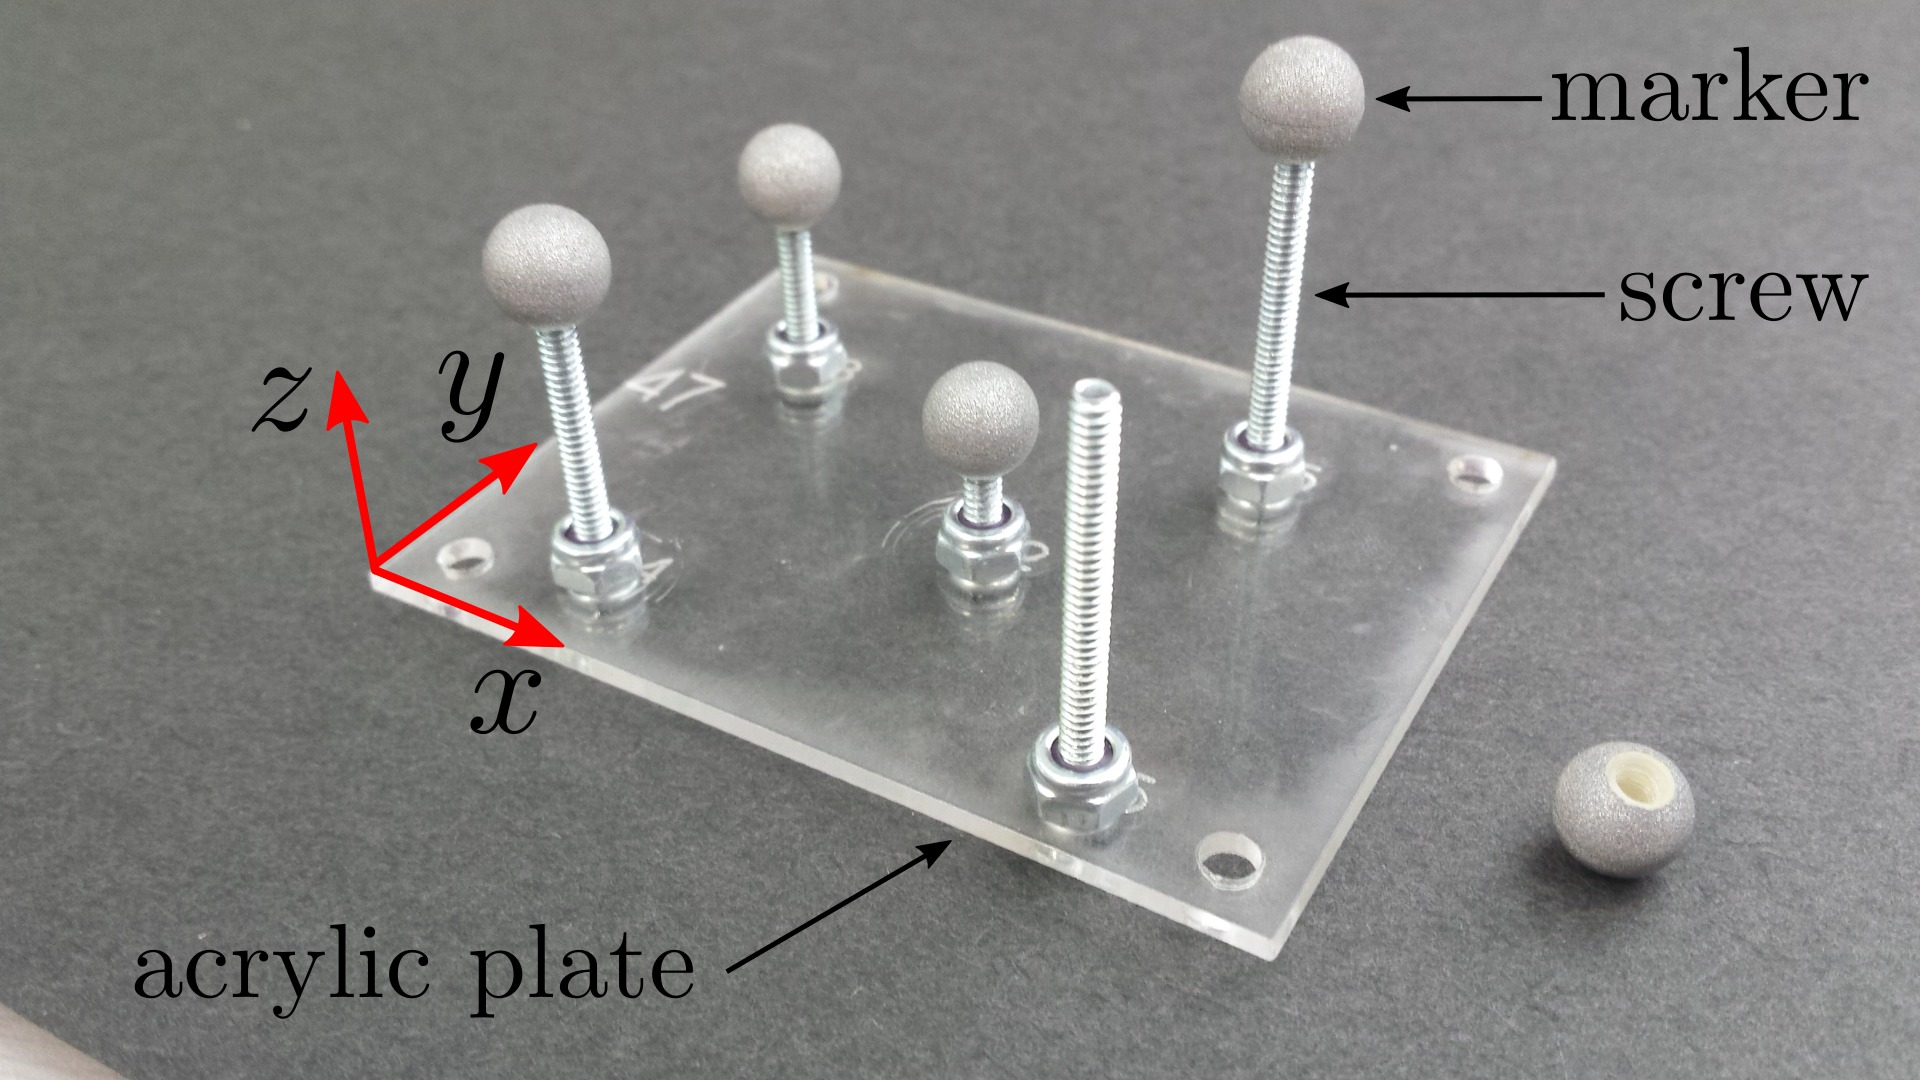
\includegraphics[width=\textwidth]{fig/hatscrews.jpg}
\caption{Vicon marker configuration}
\label{fig:hatscrews}
\end{figure}
In case the problem of finding $N$ most dissimilar configurations were solved by an optimization problem, constraints on marker configurations would further complicate the formulation. Using the approach explained above, any constraint can be enforced when the configurations are generated, obtaining, this way, only valid configurations to rank according to their similarity. This is particularly useful for the case of generating Vicon marker configurations for the following reasons. First, the distance between the centers of two markers in a configuration has to be larger than 1.5 diameters of the marker, $d$ \textbf{ref or footnote}, i.\,e. $\|x_i^{(m)}-x_i^{(n)}\|\ge1.5 d$, $\forall m,n\in{1,\ldots,M},m\neq n$. Moreover, in order to be able to build robust and reliable marker configurations in a repeatable way, instead of using rapid-prototyping techniques (e.\,g. 3D printing), we use standardized screws---which can only exist in a discrete number of lengths---onto which the markers can be mounted as in Fig.~\ref{fig:hatscrews}. This, which would have to be encoded as an integer constraint if an optimization formulation were to be used, is simply handled, in our case, by generating marker configurations which have quantized $z$-coordinates (see Fig.~\ref{fig:hatscrews}). As far as the $x$ and $y$ coordinates are concerned, there are no similar issues as the mounting holes for the screws can be automatically laser cut at any position into the acrylic transparent plate.

\section{CAD modeling}

\begin{itemize}
\item solidworks cad model
\item different configurations of the part generated from excel file (parameterized dimensions and text strings)
\item solidworks drawings
\item AI file
\end{itemize}

\section{Building the hats}

\begin{figure}
\centering
\subfloat[][Engraving hats ID and screw lengths]{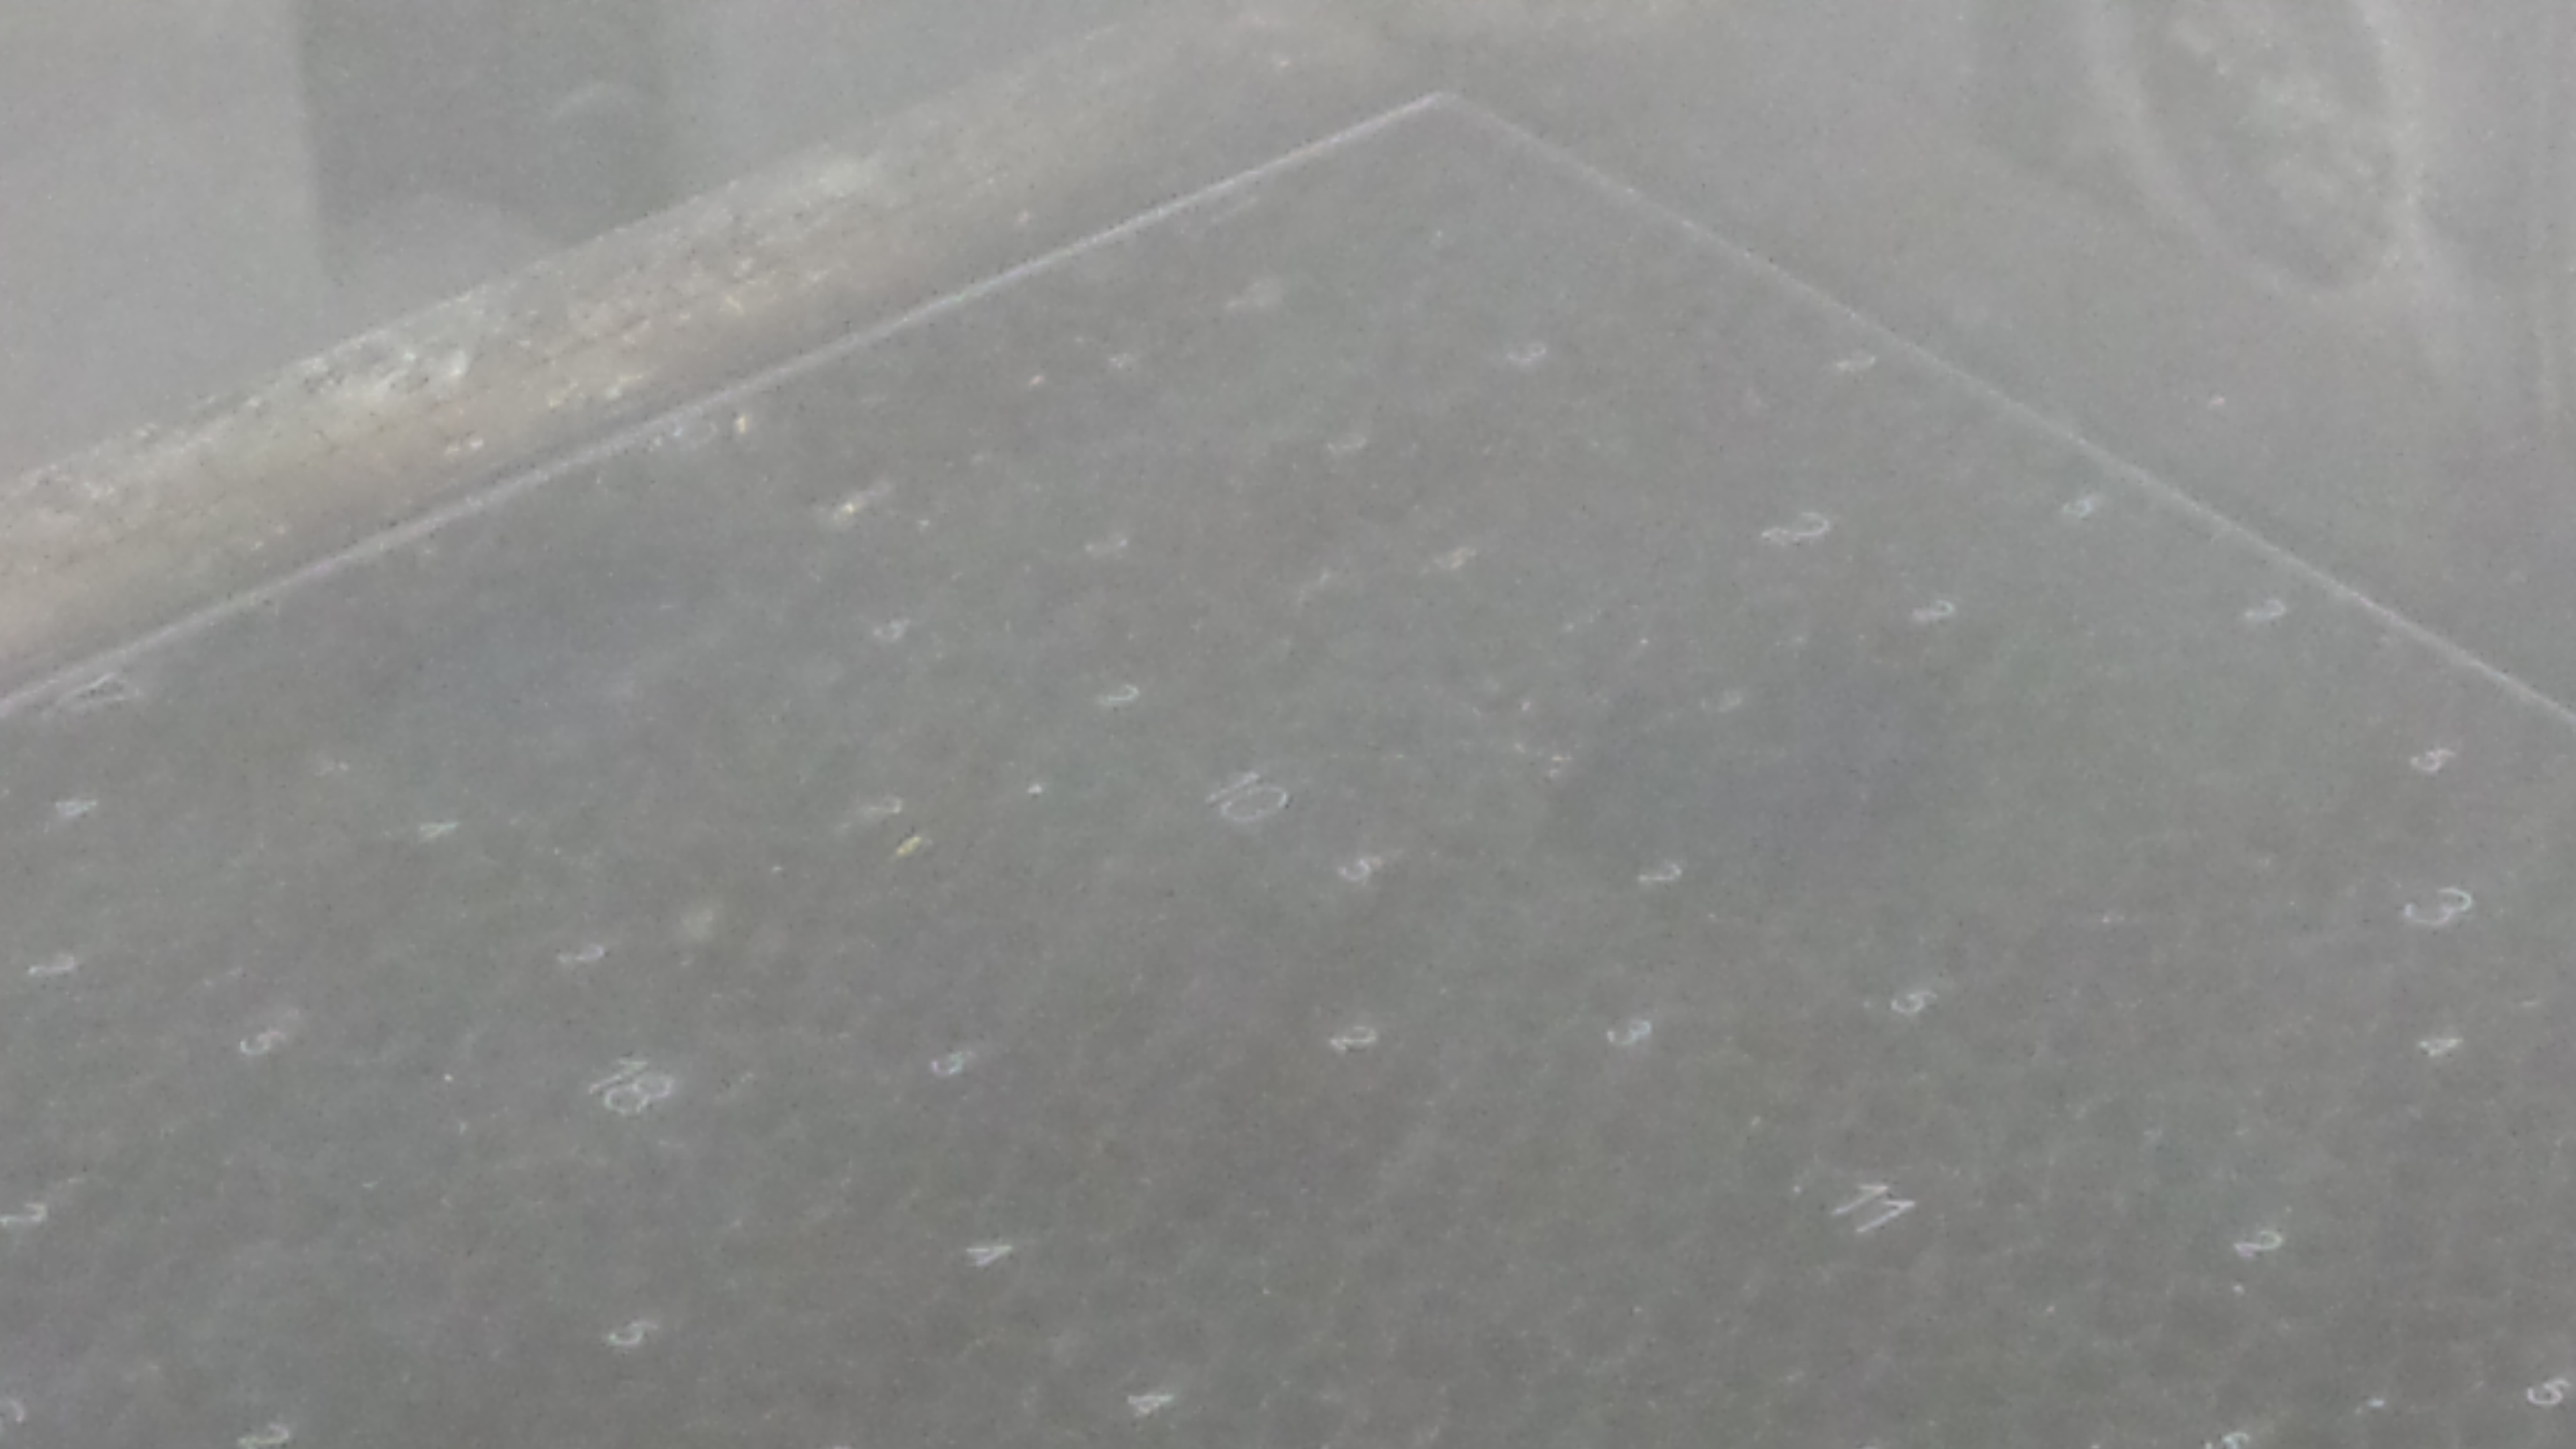
\includegraphics[width=\textwidth]{fig/laser_etching.jpg}}\\
\subfloat[][Cutting the hats]{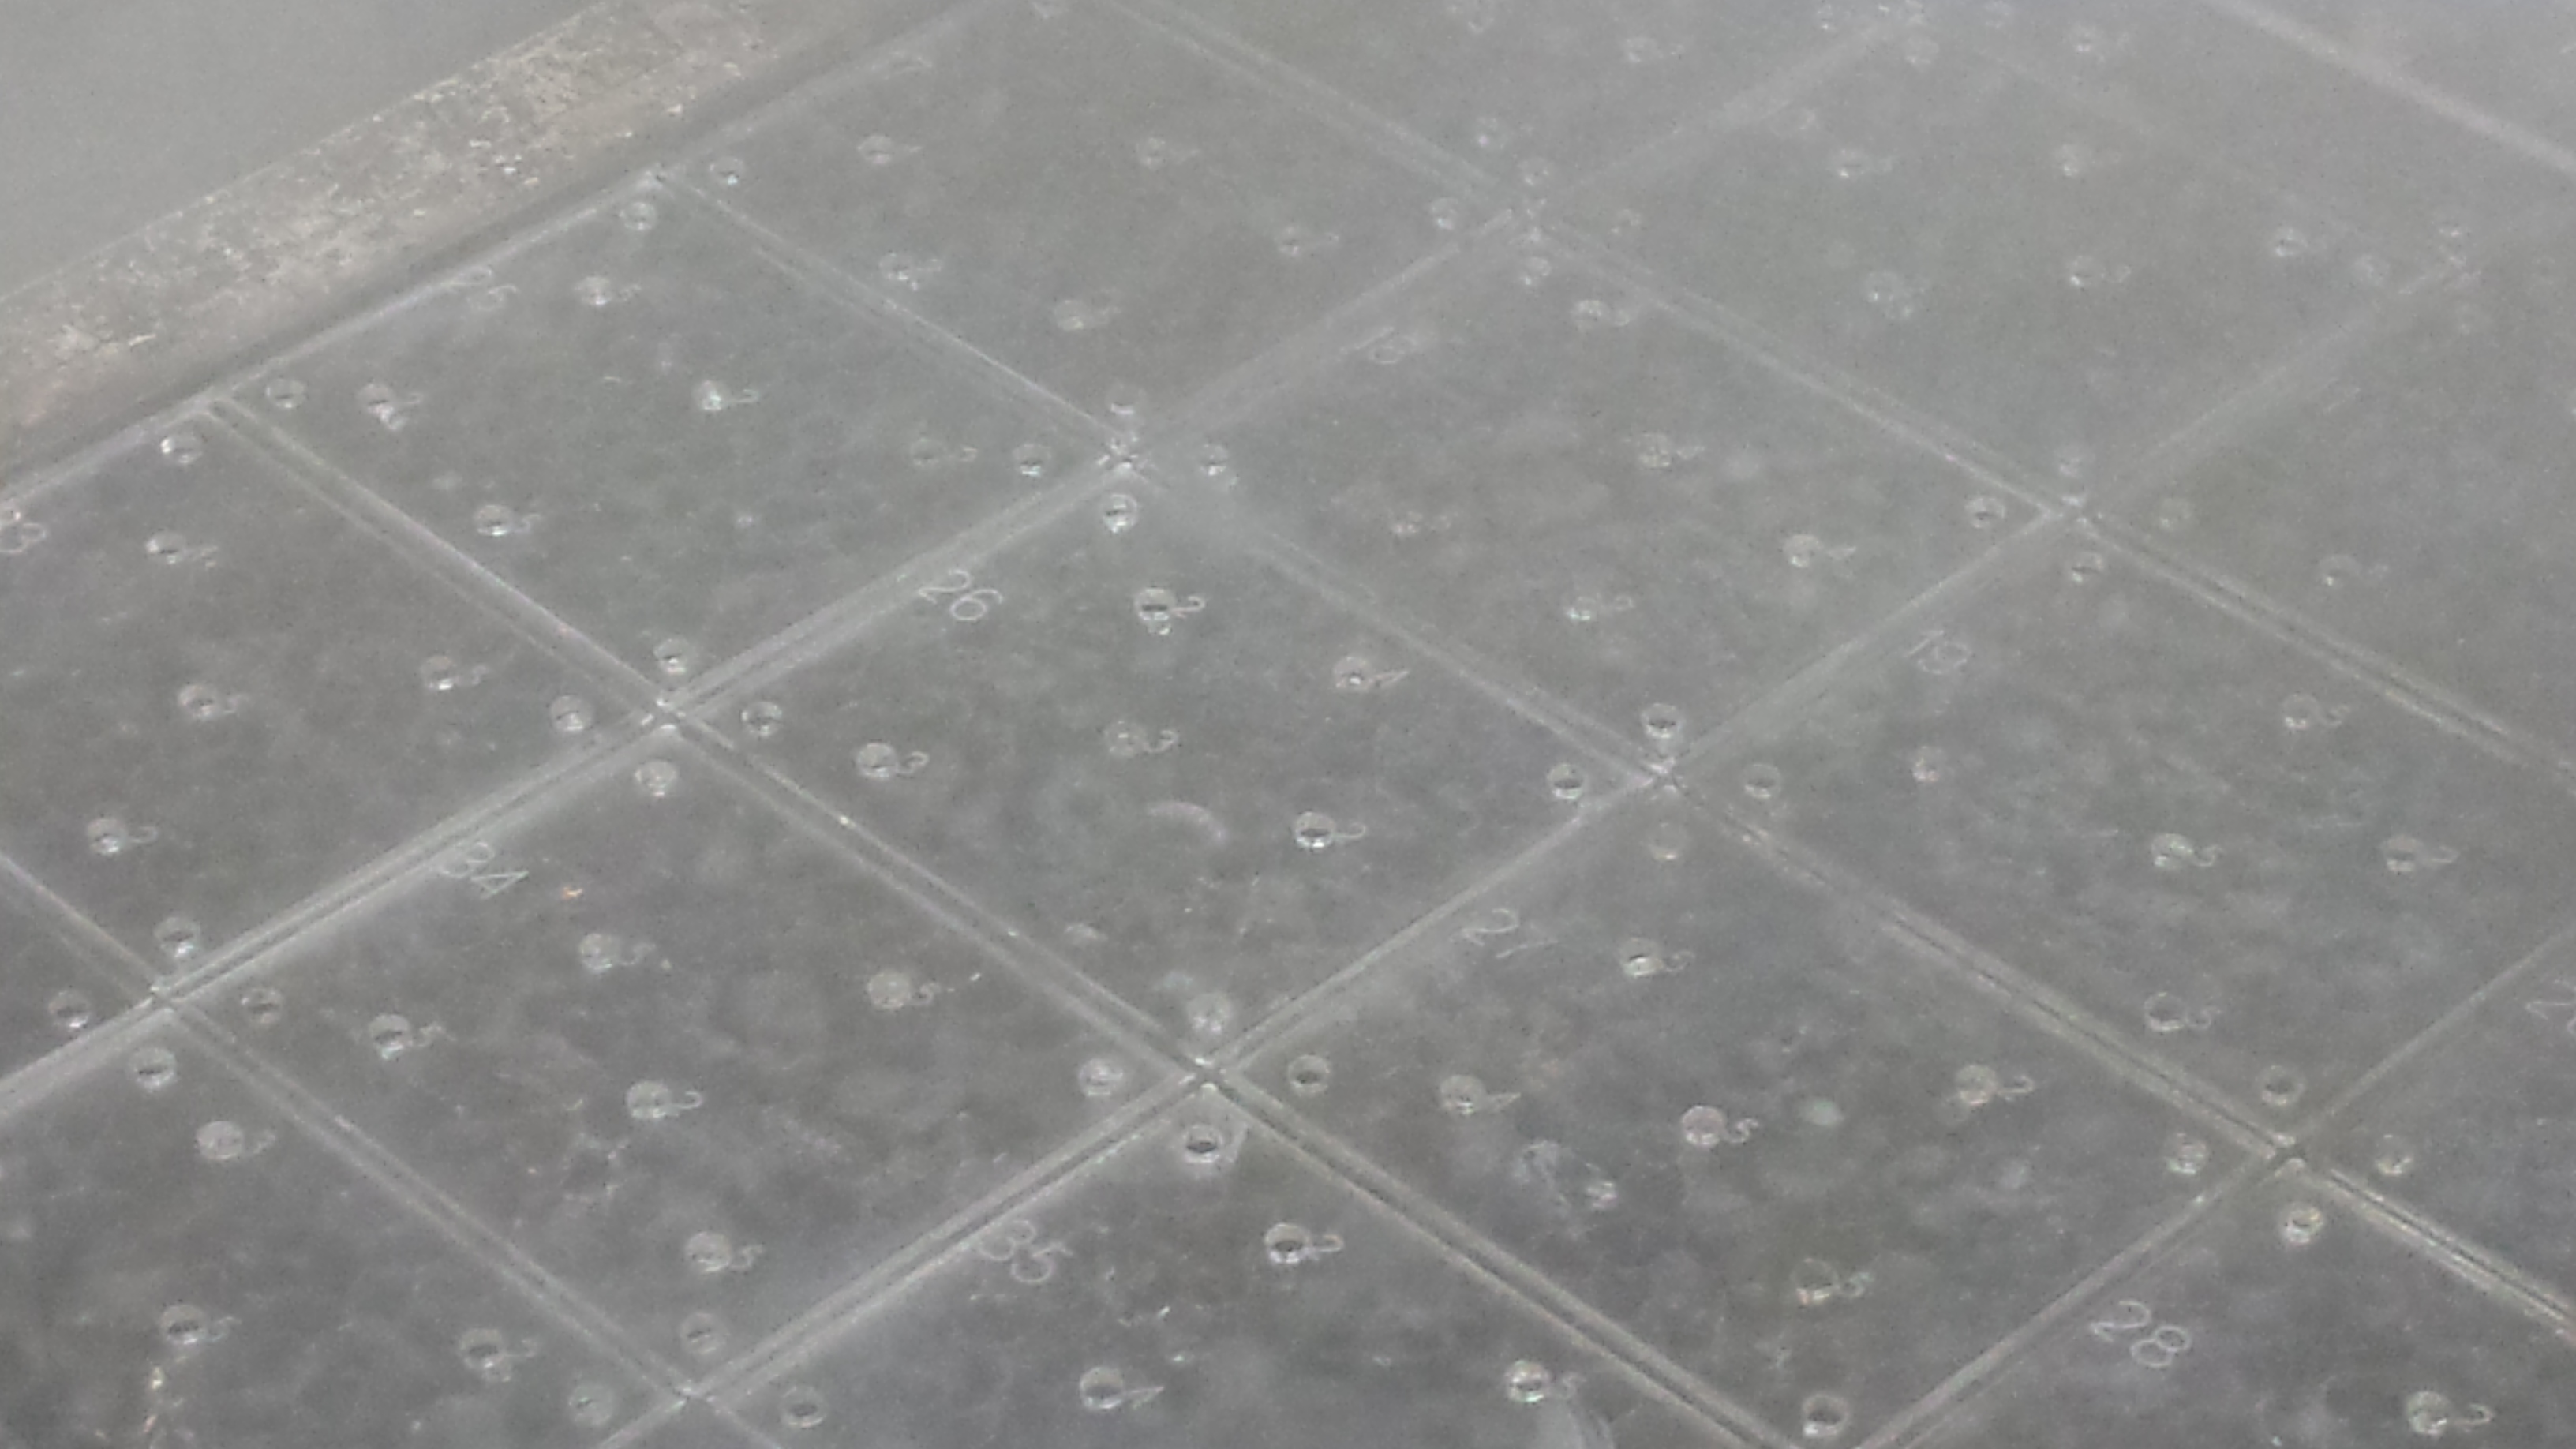
\includegraphics[width=\textwidth]{fig/laser_cutting.jpg}}
\caption{Laser cutting: engraving and etching}
\label{fig:lasercut}
\end{figure}

\begin{figure}
\centering
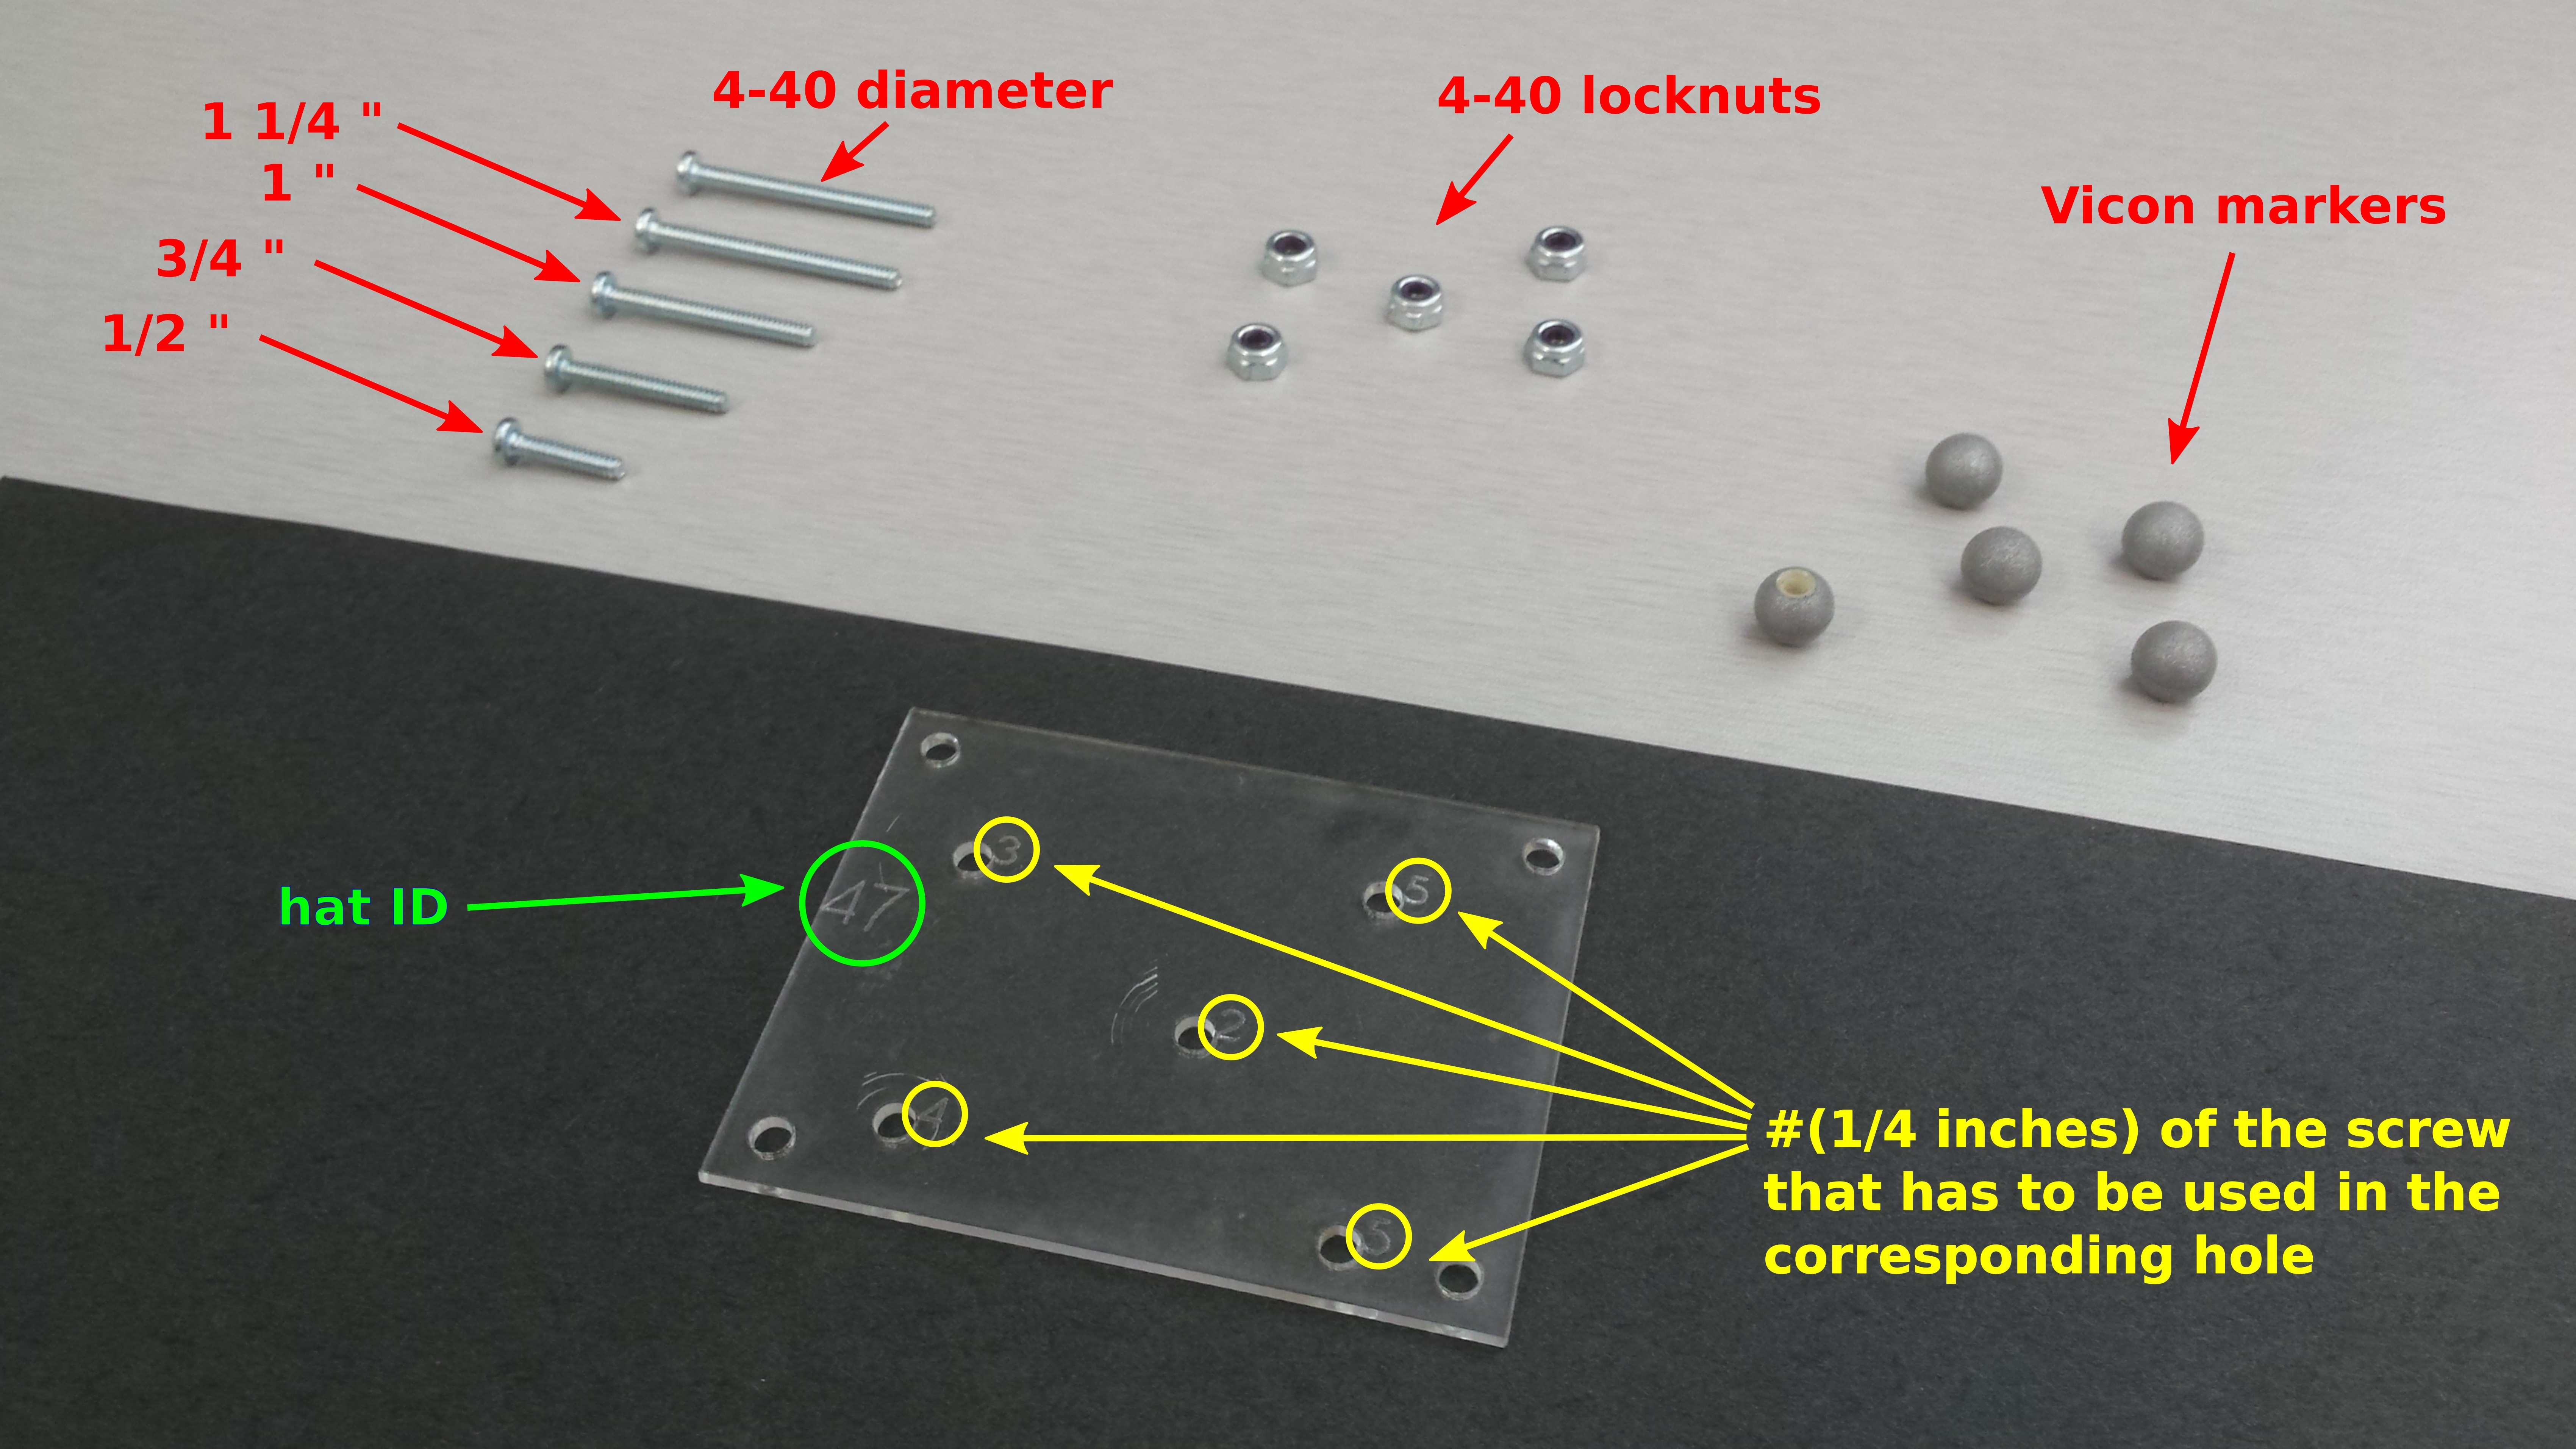
\includegraphics[width=\textwidth]{fig/assemble_parts_labeled.jpg}
\caption{Assembly parts}
\label{fig:parts}
\end{figure}

\begin{figure}
\centering
\hfill\subfloat[][Screws and locknuts]{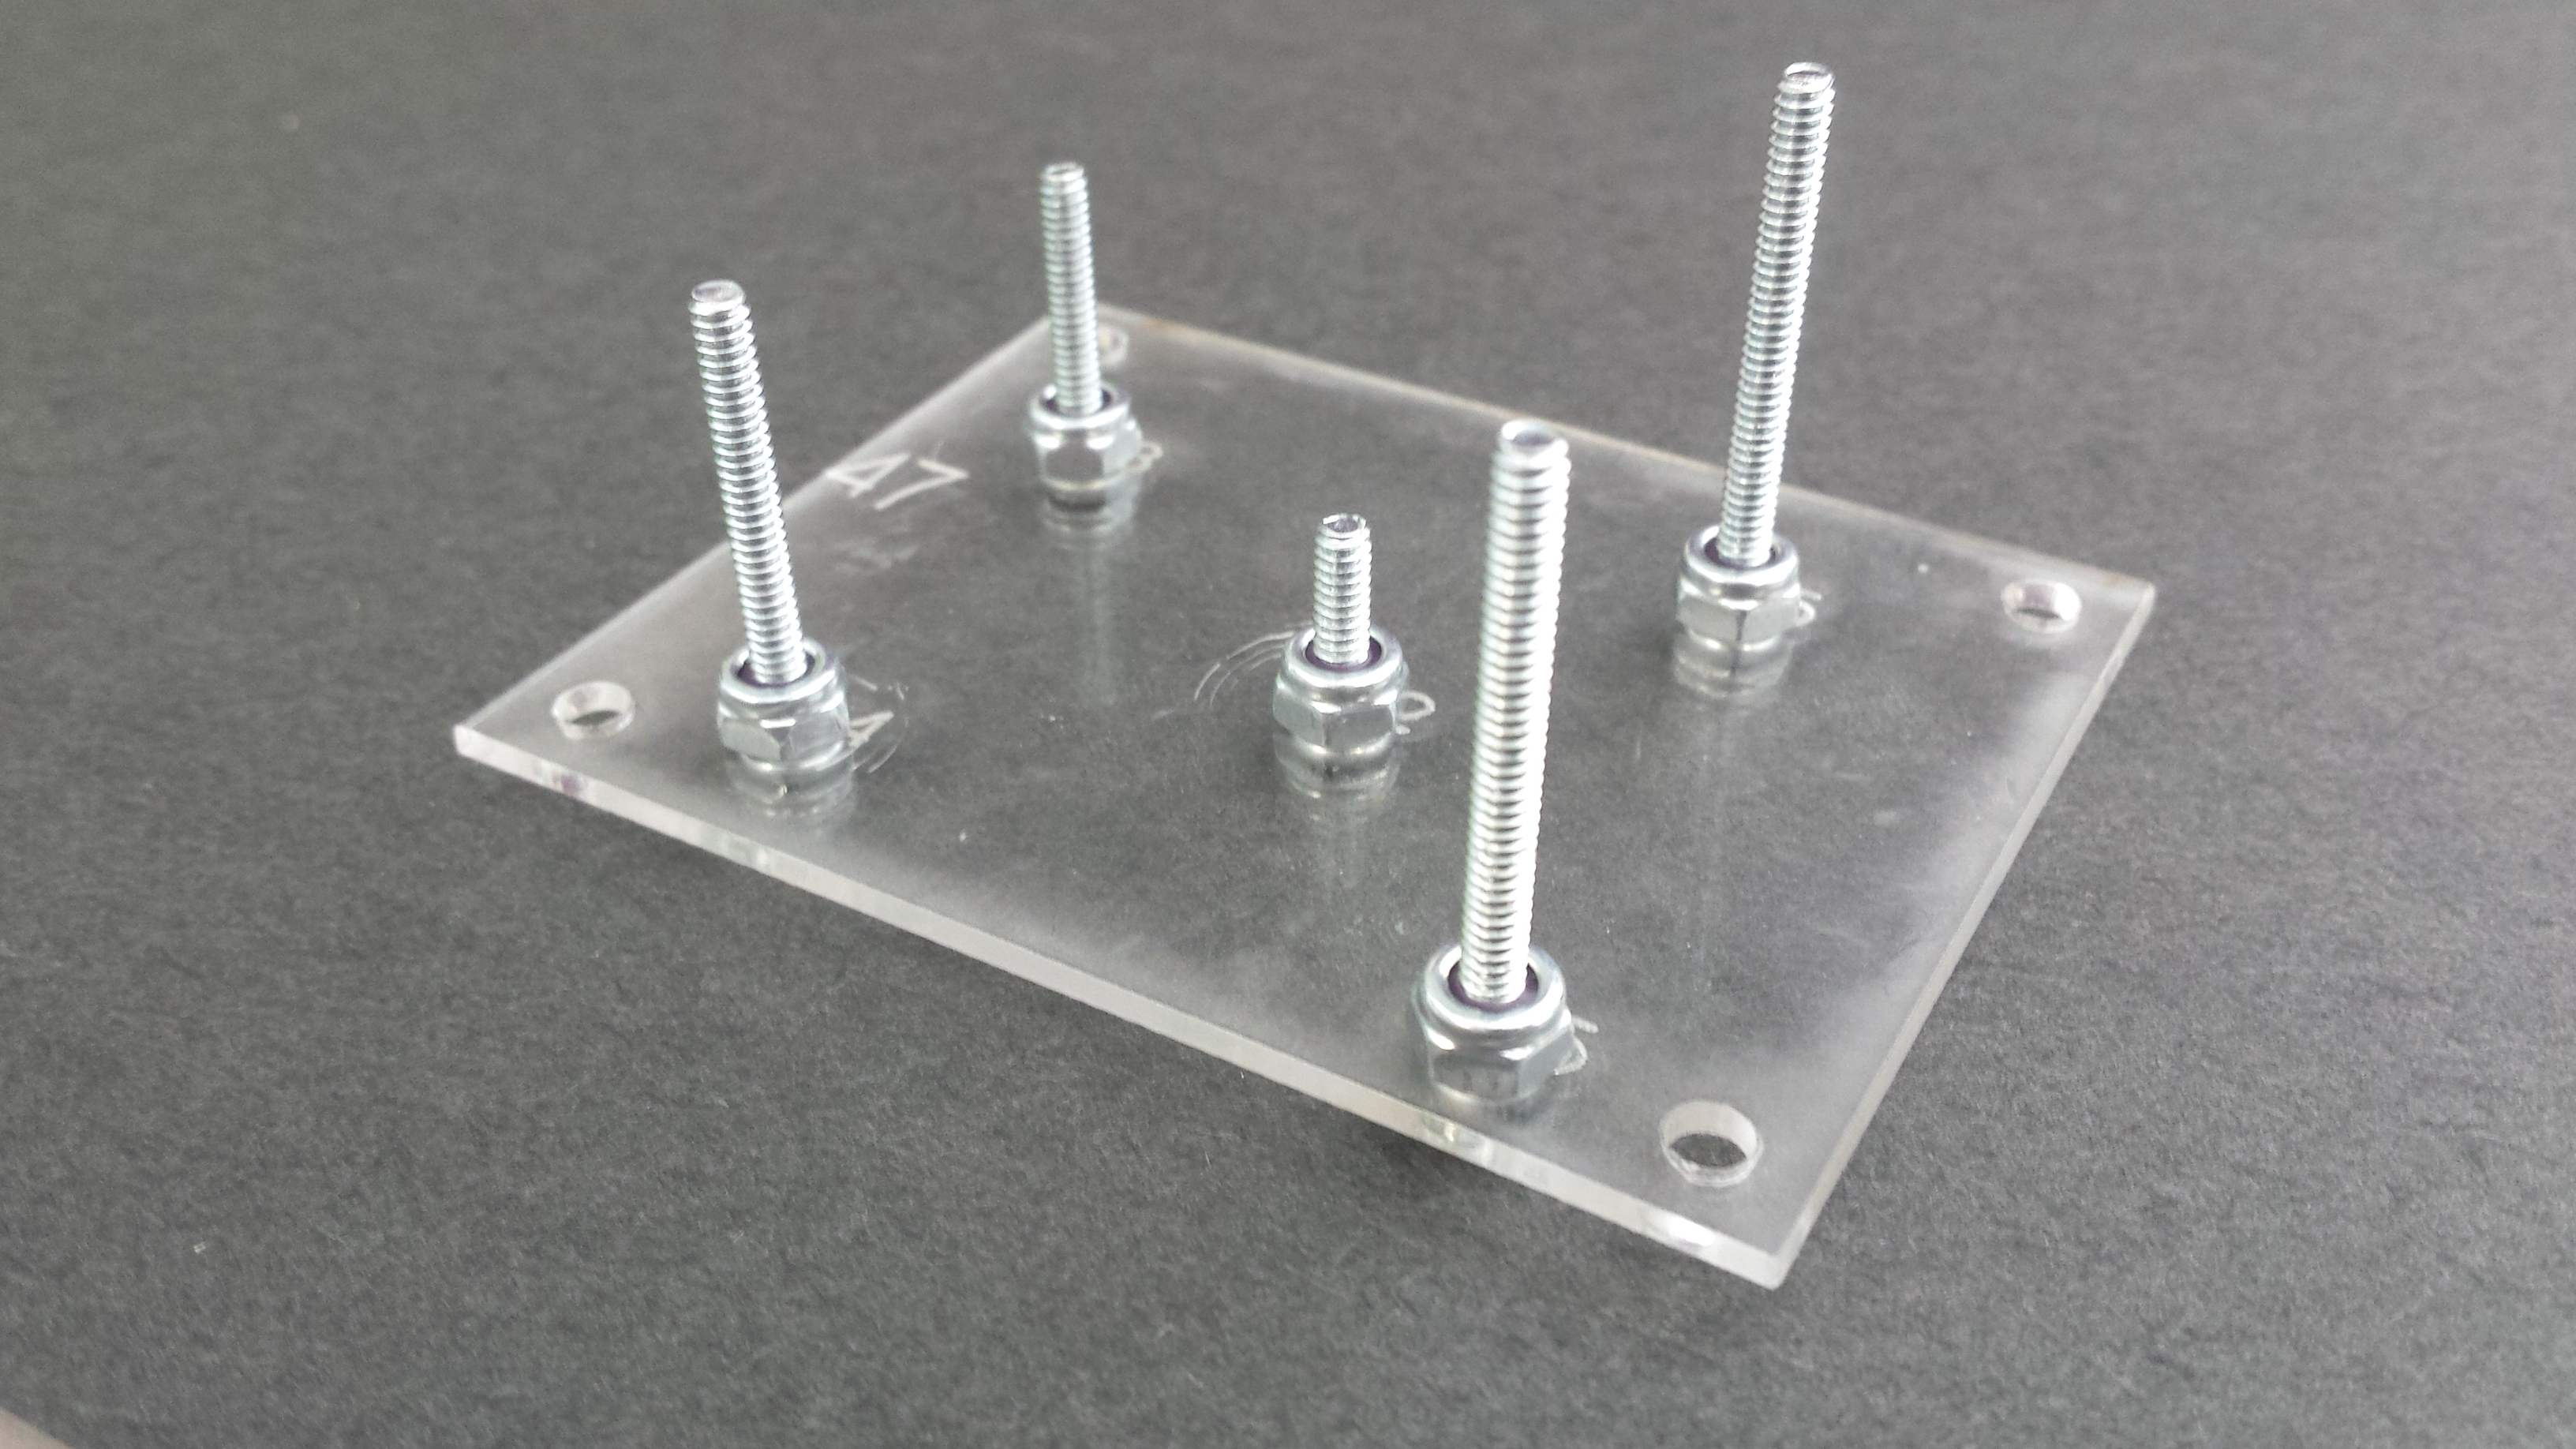
\includegraphics[trim={7cm 0cm 7cm 0cm},clip,width=0.45\textwidth]{fig/assemble_screws.jpg}}\hfill
\subfloat[][Vicon markers]{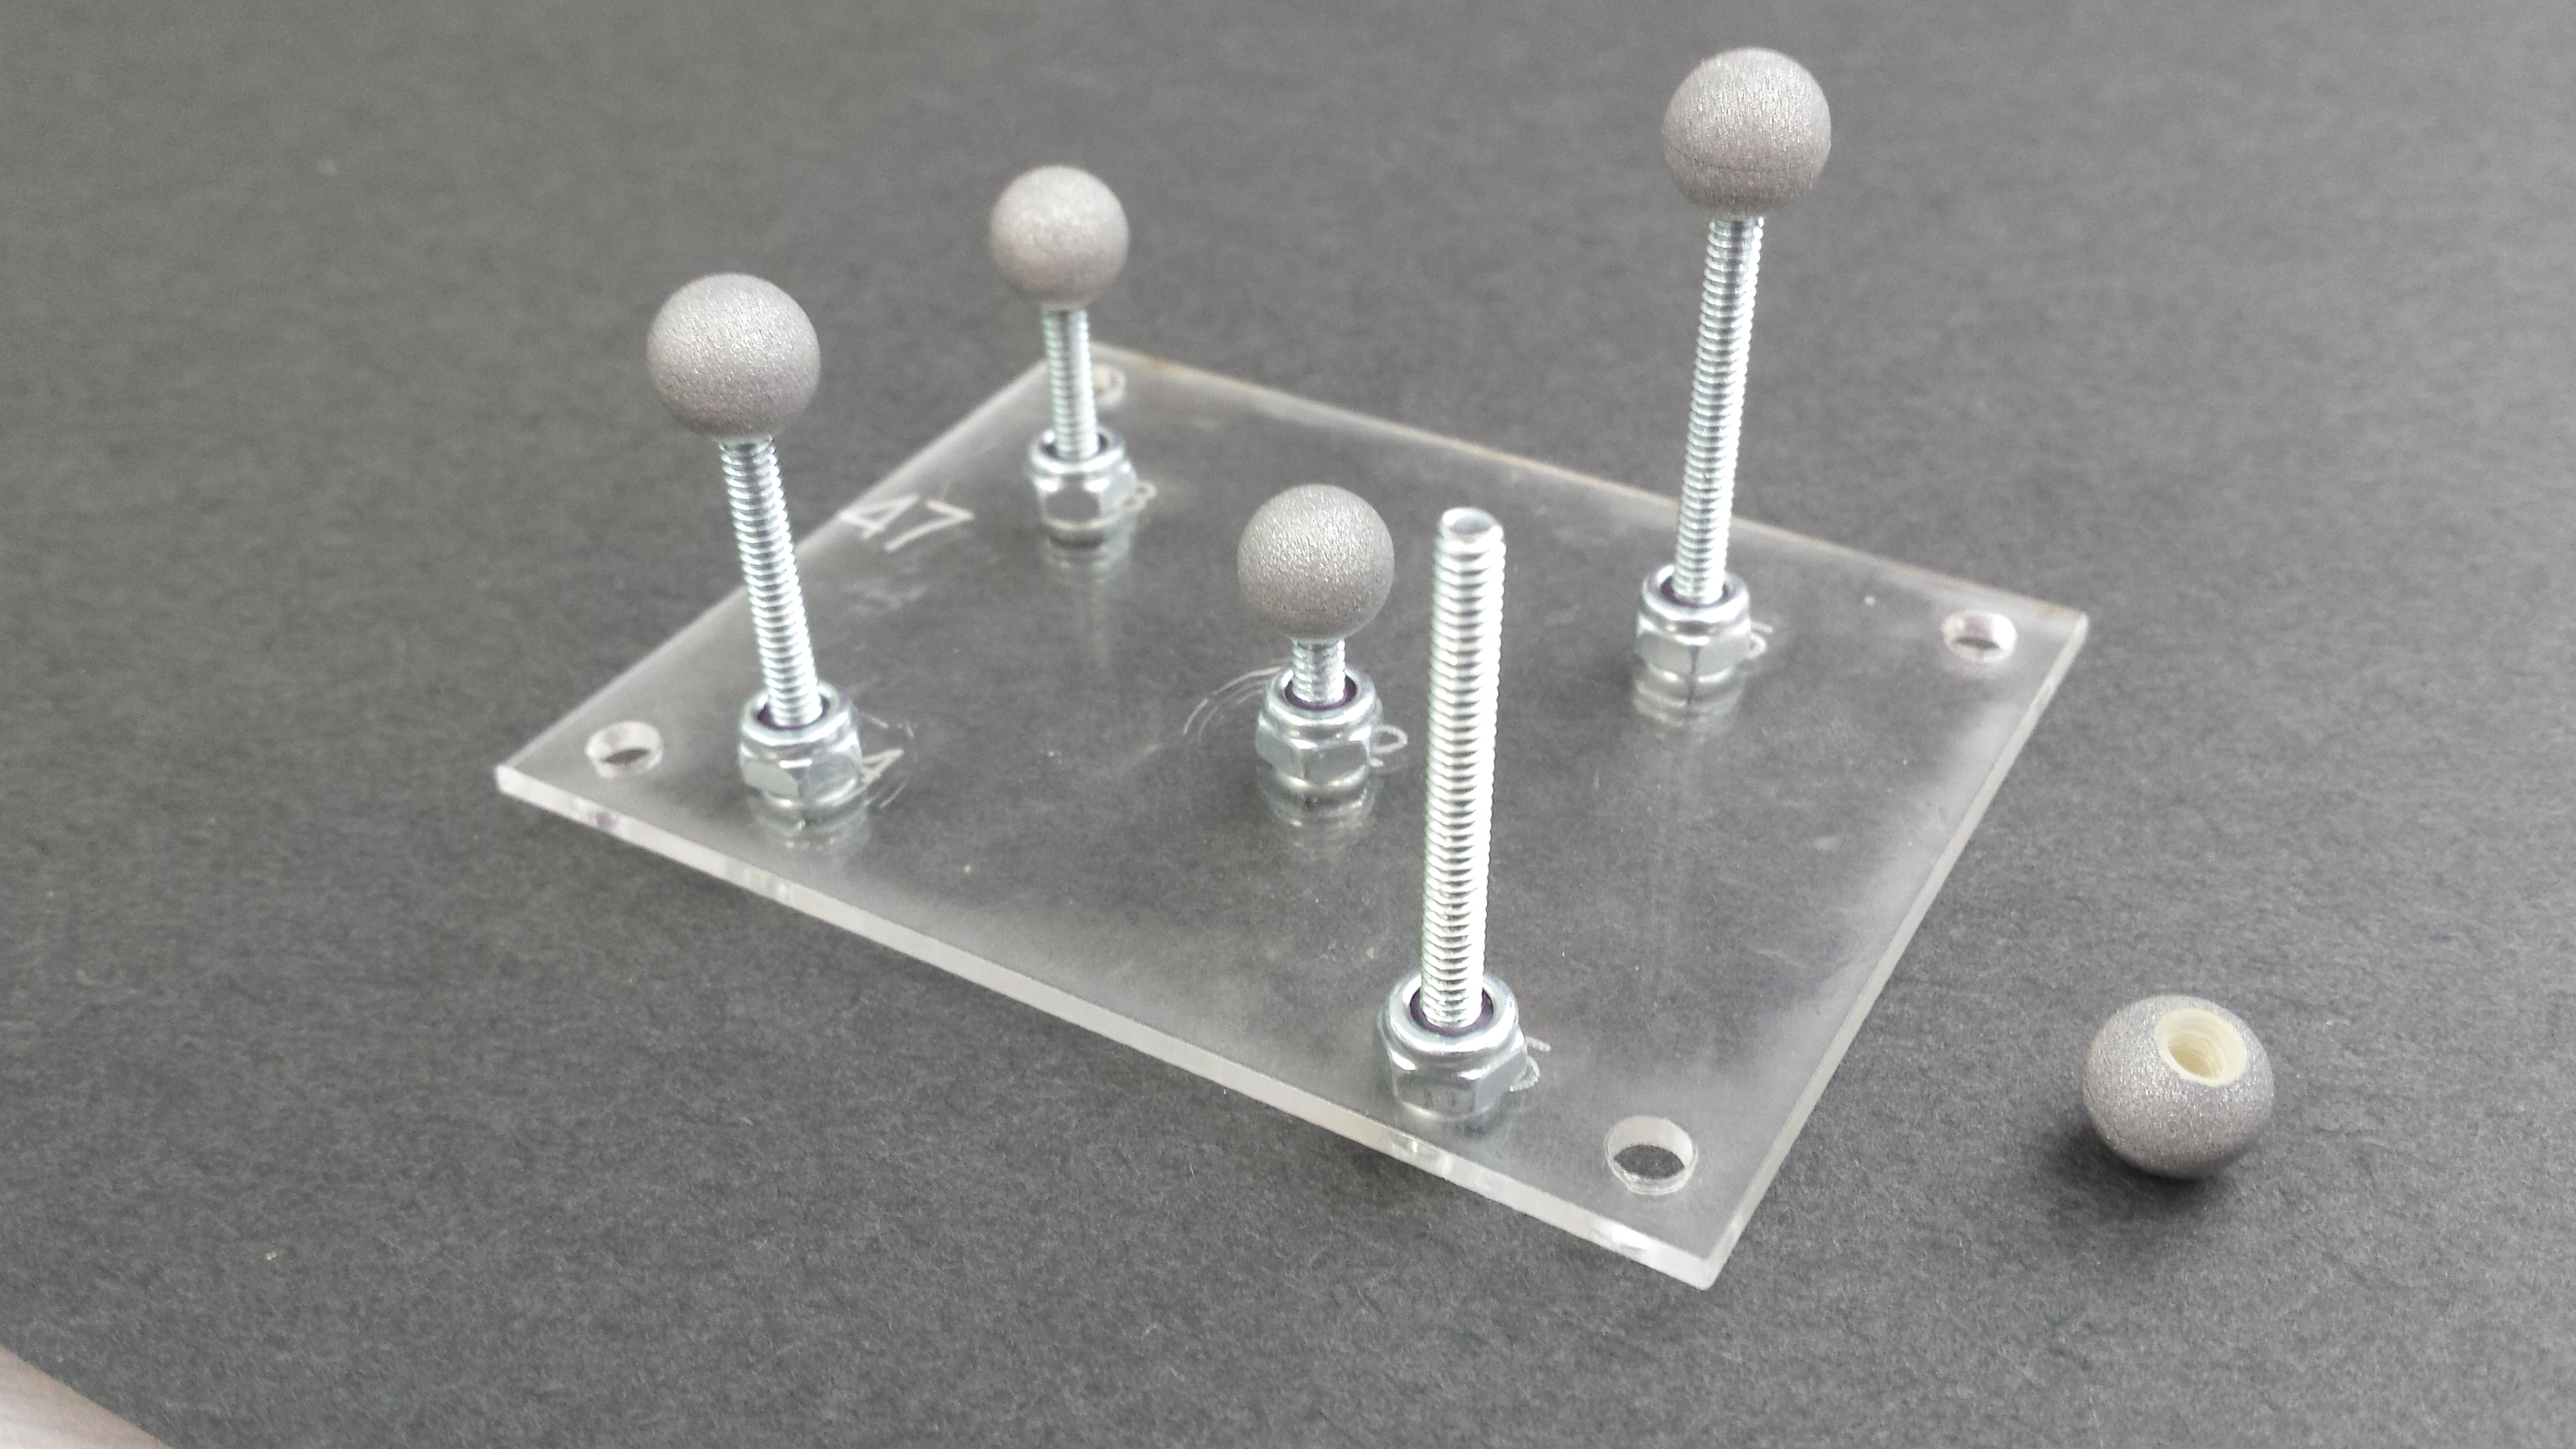
\includegraphics[trim={7cm 0cm 7cm 0cm},clip,width=0.45\textwidth]{fig/assemble_markers.jpg}}\hfill
\caption{Mounting: screws and Vicon markers}
\label{fig:mount}
\end{figure}

\bibliographystyle{unsrt}
\bibliography{bib/references}



\end{document}
